% begin module areas-ex2
\begin{frame}
\begin{example}[Example 2, p. 291]
For the region $S$ underneath the parabola $y = x^2$ from $0$ to $1$, show that the area under the approximating rectangles approaches $\frac{1}{3}$, that is,
\begin{columns}[c]
\column{.6\textwidth}
\abovedisplayskip=0pt
\belowdisplayskip=0pt
\[
\lim_{n\to\infty}R_n = \frac{1}{3}.
\]
\begin{itemize}
\item<9-| alert@9-10>  Each rectangle has width \uncover<10->{$\frac{1}{n}$.}
\item<9-| alert@11-12>  The heights are \uncover<12->{$\left( \frac{1}{n}\right)^2, \left( \frac{2}{n}\right)^2,$ $\ldots ,$ $\left( \frac{n}{n}\right)^2$.}
\item<16->  New formula:
\item<16-| alert@16-17>  $1^2 + 2^2 + 3^2 + \cdots + n^2 $ $ = \frac{n(n+1)(2n+1)}{6}$.
\end{itemize}
\column{.4\textwidth}
\only<handout:0| -1>{%
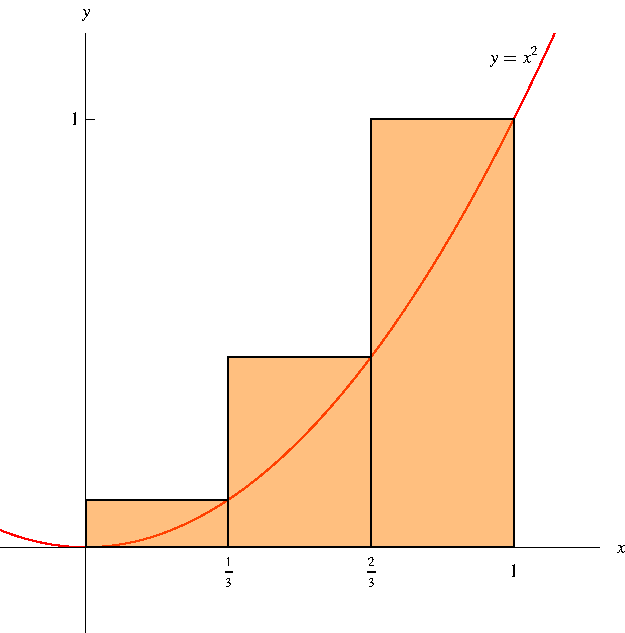
\includegraphics[height=4.5cm]{integration/pictures/05-01-righta.pdf}%
}%
\only<handout:0| 2>{%
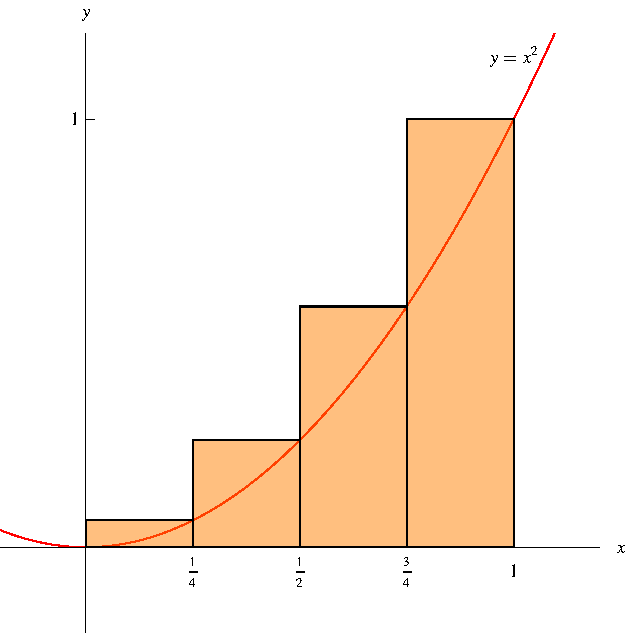
\includegraphics[height=4.5cm]{integration/pictures/05-01-rightb.pdf}%
}%
\only<handout:0| 3>{%
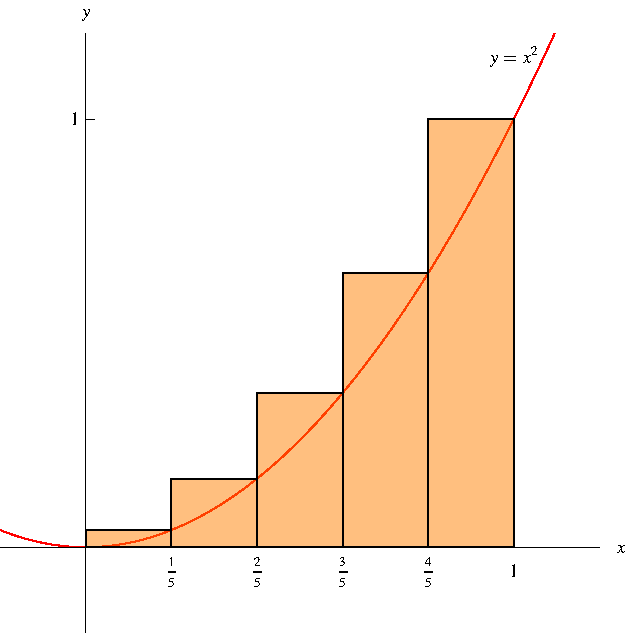
\includegraphics[height=4.5cm]{integration/pictures/05-01-rightc.pdf}%
}%
\only<handout:0| 4>{%
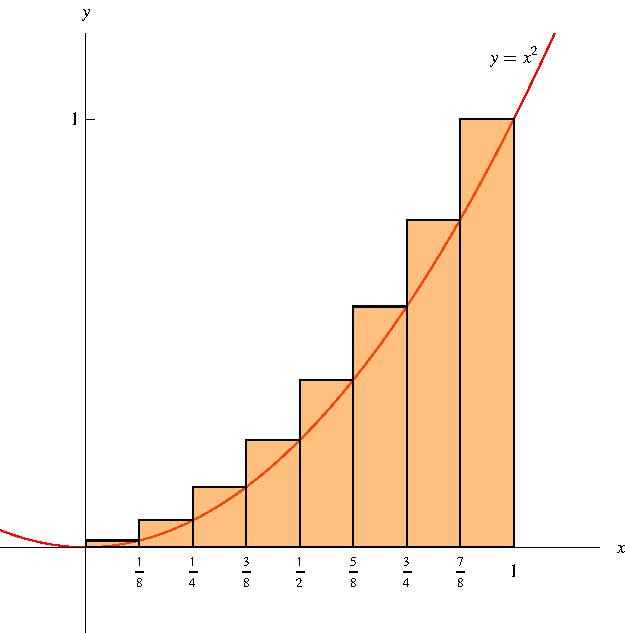
\includegraphics[height=4.5cm]{integration/pictures/05-01-rightd.pdf}%
}%
\only<handout:0| 5>{%
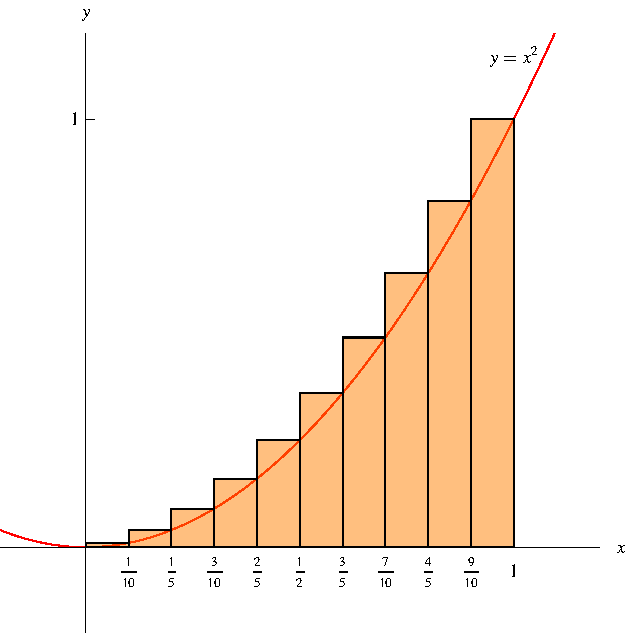
\includegraphics[height=4.5cm]{integration/pictures/05-01-righte.pdf}%
}%
\only<handout:0| 6>{%
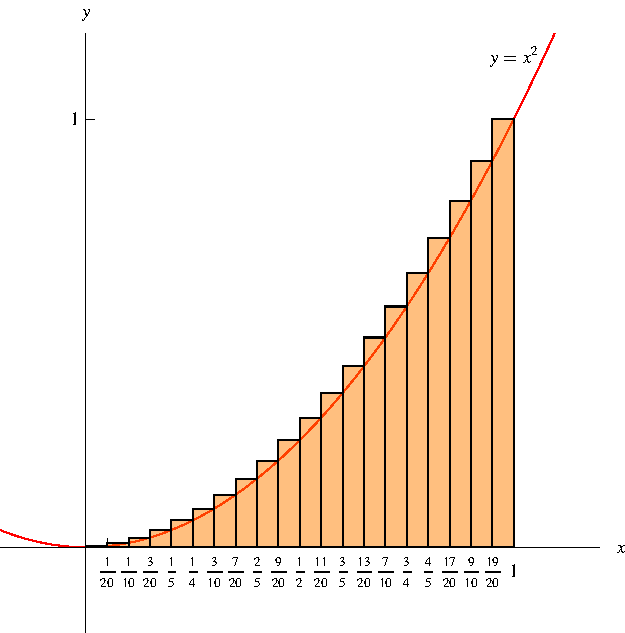
\includegraphics[height=4.5cm]{integration/pictures/05-01-rightf.pdf}%
}%
\only<handout:1-| 7>{%
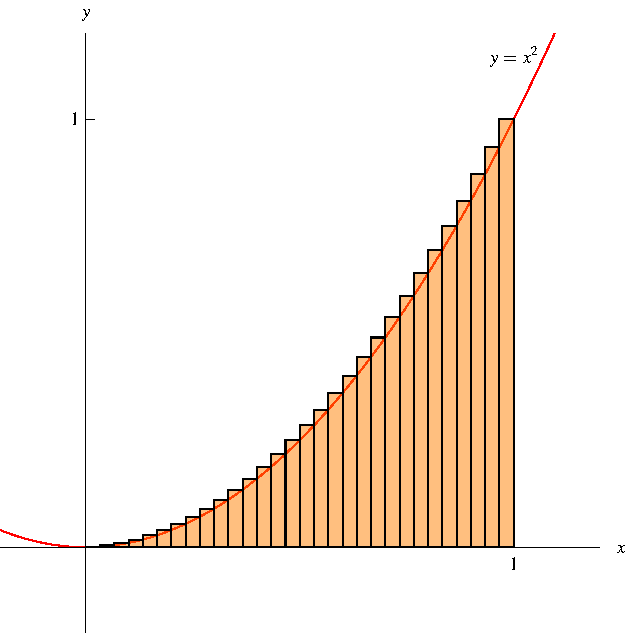
\includegraphics[height=4.5cm]{integration/pictures/05-01-rightg.pdf}%
}%
\only<handout:0| 8->{%
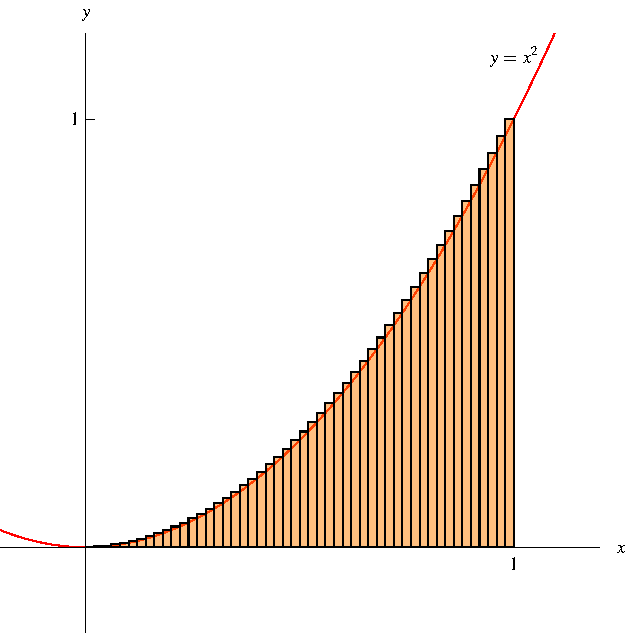
\includegraphics[height=4.5cm]{integration/pictures/05-01-righth.pdf}%
}%
\end{columns}
\abovedisplayskip=0pt
\belowdisplayskip=0pt
\[
\begin{array}{l}
\uncover<13->{%
\displaystyle R_n  =  \frac{1}{n} \left(\frac{1}{n}\right)^2%
 + \frac{1}{n} \left(\frac{2}{n}\right)^2%
 + \cdots%
 + \frac{1}{n} \left( \frac{n}{n}\right)^2%
}%
\uncover<14->{%
 = \frac{1}{n^3} \alert<handout:0| 15-17>{( 1^2 + 2^2 + \cdots + n^2)}%
}%
\\%
\uncover<17->{%
\displaystyle \lim_{n\to\infty}R_n  =  \lim_{n\to\infty}\frac{1}{n^3}%
 \alert<handout:0| 17>{\frac{n(n+1)(2n+1)}{6}}%
}%
\uncover<18->{%
 = \lim_{n\to\infty} \frac{1}{\alert<handout:0| 19>{6}} \left( 1 + \frac{1}{n}\right)\left( \alert<handout:0| 19>{2} + \frac{1}{n}\right)%
}%
\uncover<19->{%
 = \alert<handout:0| 19>{\frac{1}{3}}%
}%
\end{array}
\]
\end{example}
\end{frame}
% end module areas-ex2
